%!TEX root = ../../thesis.tex

\section{Telluric correction}
\label{sec:telluric_correction}

Typically atmospheric absorption correction has been performed by observing a standard star, a very hot (O or A-type), fast rotating star.
These stars have minimal spectral features, so reveal the atmospheric absorption when observed.
These standard stars need to be observed close in the sky and right before or after the science observation.
To have similar atmospheric absorption to the science target.
The science target can be corrected for the telluric line by division by the telluric standard star~\citep[e.g.][]{vacca_method_2003}.
For high-resolution spectroscopy this technique is not sufficient to correct telluric with residuals greater than 2\% remaining.

Recently synthetic modelling of telluric absorption has gained popularity with several works focusing on correcting telluric absorption with synthetic models~\citep[e.g.][]{bailey_correcting_2007, cotton_atmospheric_2014, seifahrt_synthesising_2010} and achieving better correction than the standard star method.
Several different software available which usually build upon the standard line-by-line radiative transfer model code {LBLRTM}~\citep{clough_linebyline_1995}.
Some examples are {TelFit}~\citep{gullikson_correcting_2014}, and ESO's {Molecfit}~\citep{smette_molecfit_2015} which both model and fit a synthetic absorption spectra to observations, where as {TAPAS}~\citep{bertaux_tapas_2014} just creates synthetic models based on atmospheric data for an observation (without fitting).
The synthetic models at high resolution are very sensitive to atmospheric constituents, especially water vapour, and observing conditions such as the airmass.

Recently~\citet{ulmer-moll_telluric_2018} compared the telluric correction efficiency between {TelFit}, {Molecfit}, {TAPAS}, and the standard star method.
They found that {Molecfit} and {Telfit} synthetic corrections lead to smaller residuals for lines arising from \ce{H2O}, while the standard star method corrects for \ce{O_2} lines best.
All methods (synthetic and standard star) result in a scatter inside the telluric lines of 3--7\%.
They also find that an observatory tailored atmospheric profile leads to reduced scatter inside telluric lines and that the correction performed better with lower precipitable water vapour.

As an example \cref{fig:telluricmodelcomparision} shows the telluric correction using the three different methods, {Molecfit}, {TelFit} and {TAPAS}\footnote{Performed here by Sol\`{e}ne Ulmer-moll.}, of a spectrum extracted for this work, detector \#4 of observation HD\,4747-1  (see \cref{tab:observations}).
There are differences between the models of around 2\% level, with the largest difference near the deep telluric line around 2163\nm{}.
\begin{figure}
    \centering
    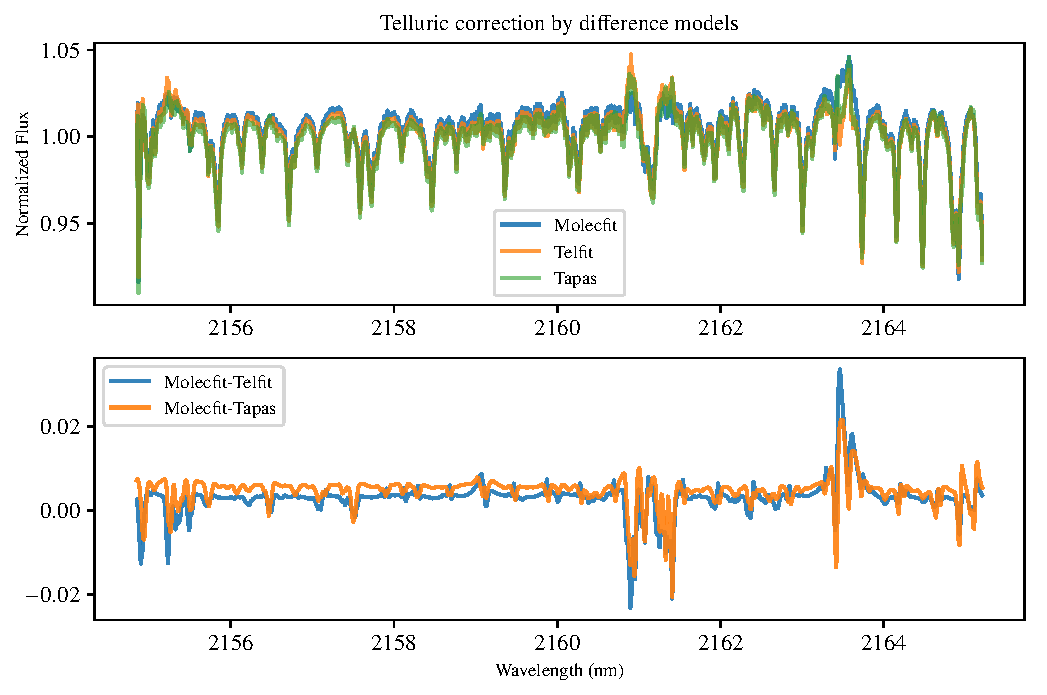
\includegraphics[width=0.7\linewidth]{figures/atmos_and_models/Telluric_model_comparision}
    \caption{CRIRES spectra with telluric correction applied using the {Molecfit}, {TelFit} and {TAPAS}.
        Top: The telluric corrected spectra.
        Bottom: Difference between the corrected spectra from the different methods.}
    \label{fig:telluricmodelcomparision}
\end{figure}

Since sufficient telluric correction can be achieved through synthetic modelling, the observational requirement is halved as the standard star is not required, allowing more observing time for science.
This is the case with the CRIRES observations analysed in this work.
This work utilizes the synthetic spectra produced from {TAPAS} models are used correction the telluric lines in CRIRES spectra.
These are detailed further below.

\subsection{{TAPAS} web service}
\label{subsubsec:TAPAS}

Telluric absorption spectra can be obtained with the {TAPAS} (Transmissions of the AtmosPhere for AStronomical data) web service\footnote{\href{http://cds-espri.ipsl.fr/tapas}{http://cds-espri.ipsl.fr/tapas}}~\citep{bertaux_tapas_2014}.
{TAPAS} uses the standard line-by-line radiative transfer model code LBLRTM~\citep{clough_linebyline_1995} along with the 2008 {HITRAN} spectroscopic database~\citep{rothman_hitran_2009} and {ARLETTY} atmospheric profiles derived using meteorological measurements from the ESPRI data centre\footnote{\href{https://cds-espri.ipsl.upmc.fr}{https://cds-espri.ipsl.upmc.fr}} to create telluric line models.

The {ARLETTY} atmospheric profiles have a 6~hour resolution, so there may be a slight difference between the actual profile at the time of observation.

There are several parameters that can be submitted to the web service to define the requested telluric spectra, such as: target coordinates, date and time, location, spectral resolution, wavelength range and units choice observations, as well as the atmospheric profile and the choice of several atmospheric constituents to be included in the model spectra. {TAPAS} produces the telluric spectrum and sends a link to the results via email.


\subsection{Requests for this work}
Synthetic telluric absorption were requested from the {TAPAS} web service for this work.
These were to match the CRIRES observations which are presented in \cref{tab:observations}.

The mid-observation time for each observation was used to request a synthetic spectra individually for each observation, with the {ARLETTY} atmospheric profiles and vacuum wavelengths selected.
The telluric models were retrieved without barycentric correction to keep the telluric lines at a radial velocity of zero with respect to the instrument.
For each observation one model was requested with all available atmospheric species present, convolved to a resolution of \(\rm R=50\,000\), and a further two models without the instrumental profile convolution applied.
For these two extra models, one contained only the transmission spectra of \ce{H2O} while the other contained contributions from the all other constituents except \ce{H2O}.
This was to explore a known issue with the depth of \ce{H2O} absorption lines in the {TAPAS} models~\citet{bertaux_tapas_2014} (see \cref{subsec:telluric_correction_application}).
An example of the telluric spectrum for the \ce{H2O} and the non-\ce{H2O} species is given in \cref{fig:telluriccomponents}. To obtained a combined model of all species these two can be multiplied together.

\begin{figure}
    \centering
    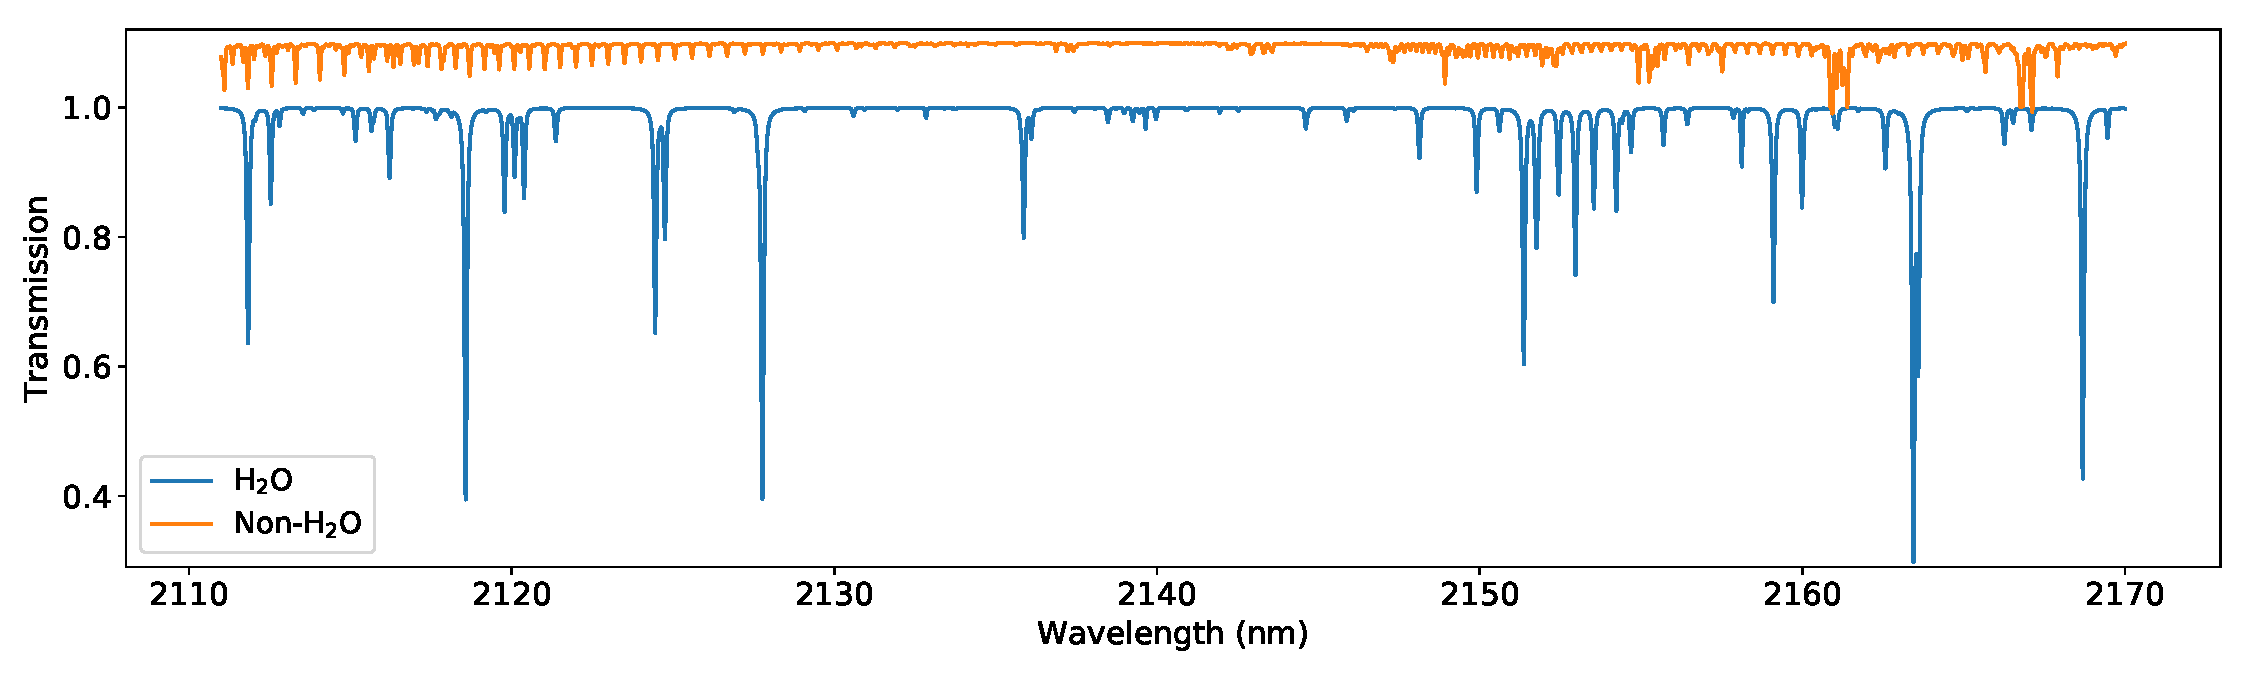
\includegraphics[width=0.9\linewidth]{figures/atmos_and_models/telluric_components}
    \caption{Telluric absorption spectrum for \ce{H2O} and the non-\ce{H2O} species available from {TAPAS}. In the wavelength range 2110--2170\nm{} and both at a resolution of 50\,000. A vertical offset of 0.1 has been added to the non-\ce{H2O} spectrum.}
    \label{fig:telluriccomponents}
\end{figure}


\subsection{Issues with {TAPAS}}
There are a number of issues encountered when using the {TAPAS} web service, mainly due to interaction with the website.
Often their service were down for weeks at a time without any warning or notification.
With this, time was wasted filling out and submitting a requests via the the web form without a response, or a returned spectra.
There was also a variable level of success between different web browsers.
A number of bug reports were submitted to the owners of the webpage without any acknowledgement.

The webpage is useful for quickly obtaining a small number of spectra but can be tedious for many spectra.
For this work this was around upwards of 50 telluric spectra, (3 for each of the 17 observations).
{TAPAS} offers the ability to request multiple spectra at a time but this was found to be unreliable when attempting to request more than four spectra in a single request.

A script\footnote{Available at \href{https://github.com/jason-neal/equanimous-octo-tribble/blob/master/octotribble/Tapas/}{https://github.com/jason-neal/equanimous-octo-tribble/blob/master/octotribble/Tapas/}} was created to automatically generate the data necessary to fill out a {TAPAS} request for each {CRIRES} observations.
The script scanned the {CRIRES} header for information such as the mid-time of observations, target coordinates, slit width etc.\ and populated the {XML} request form provided by {TAPAS}.
The script output is copied and pasted into the web browser for submission.

Trial and error was needed to understand all the {XML} form entries, such as the molecules requested and the atmospheric model to use ({ARLETTY}) and achieve a valid {TAPAS} request.
The real issue was with the {TAPAS} {{ID}} number.
Each {TAPAS} request has an {ID} number (which is provided with the email response).
This {ID} number needs to be correctly set in the {XML} form before submission.
This number is incremented by 1 with each submission but its initial value is unknown unless you made the very last request.
If a submission is made via the {XML} request with the incorrect {ID} number a response will be returned with the correct {ID} number, but the failed request will be returned.
This can then be used to increment the {ID} number by 1 and hopefully make a valid request.
Unfortunately, if another user makes a {TAPAS} request between submissions the {ID} number will again be invalid.
It is unknown if multiple transmission spectra could have been requested at the same time with the {XML} form.

There is another issue with a one hour time offset between the requested and the time returned by {TAPAS}.
For instance if the requested time was for an observation at 0200h {UTC} then the transmission spectrum returned by {TAPAS} is for 0100h {UTC}.
This changes the position of the target, the airmass and potentially the {ARLETTY} model used (6 hour time steps), affecting the strength of the telluric lines.
It is tedious to remember to offset your input time by one hour to obtain the correct time, and slightly more work when you also have to adjust the date when going backwards past 0000h.
When submitting the {XML} script the time that is returned is the time requested.
Attempts were made to bring this issue to the attention of the {TAPAS} team in 2016 but as of August 2018 this issue is still present.

These issues need to be considered when requesting {TAPAS} spectra, adding unnecessary difficultly to the relatively simple process.


\subsection{Telluric masking}
The telluric spectra from {TAPAS} can not only be used for correcting individual spectra but are also easily used to create a wavelength mask telluric lines.For instance~\citet{figueira_radial_2016} and~\citet{artigau_optical_2018} use {TAPAS} spectra to mask out atmospheric lines deeper than 2\% for computing the photon noise limited radial velocity precision.
A telluric wavelength mask is similarly used in \cref{cha:nir_content} when extending the analysis of~\citet{figueira_radial_2016}.
The telluric model used for this is an average of 52 {TAPAS} spectra (one per week in 2014), simulated at La Silla Observatory at an airmass of 1.2 (\(z = 33.5^{o}\)).
This is to incorporate long-term variations of absorption over the year.
Masking is applied by defining a cut-off line depth, typically 2\%, at which to mask out any deeper lines.
